\documentclass[30pt,twocolumn,letterpaper]{article}
\usepackage{cvpr}
\usepackage{times}
\usepackage{booktabs}
\usepackage{epsfig}
\usepackage{graphicx}
\usepackage{amsmath}
\usepackage{amssymb}
\cvprfinalcopy
\def\cvprPaperID{****}
\def\httilde{\mbox{\tt\raisebox{-.5ex}{\symbol{126}}}}
\usepackage{graphicx}
\usepackage{indentfirst}
\setlength{\parindent}{2em}
\usepackage{cite}
\usepackage[colorlinks,linkcolor=red,anchorcolor=blue,citecolor=green,backref=page]{hyperref}
\author{Qilei Zhang\\\\
Jun 30 2018}
\title{Generating Sentences from Images}
\begin{document}
\maketitle
\begin{abstract}
  Humans can prepare concise descriptions of pictures, focusing on what they find important.
\end{abstract}
\section{Introduction}
This paper describes a system that can calculate the image of a score connected to a sentence. This score can be used to attach descriptive sentences to a given image, or to get an image of a given sentence. For most pictures, humans can prepare a concise description in the form of a sentence relatively easily\cite{Agrawal2012Data}. Such descriptions might identify the most interesting objects, what they are doing, and where this is happening. These descriptions are rich, because they are in sentence form. They are accurate, with good agreement between annotators\cite{Javorszky2003Information}. \\
\begin{figure}[htbp]
\small
\centering
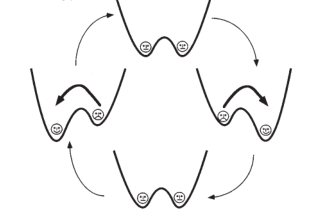
\includegraphics[width=20em]{000.png}
\caption{There is an intermediate space of meaning which has different projections to
the space of images and sentences. Once we learn the projections we can generate
sentences for images and find images best described by a given sentence.}
\label{fig:lable}
\end{figure}\\
\section{Authors Suppressed Due to Excessive Length}
Sentences can describe the same phenomena. Synecdoche and the general richness of vocabulary means that many different words can quite legitimately be used to describe the same picture\cite{Kakumanu2006A}.\\
\begin{figure}[htbp]
\small
\centering
\includegraphics[width=20em]{001.png}
\caption{Multi-task Network Cascades for instance-aware semantic segmentation. At the top right corner is a simplified illustration.}
\label{fig:lable}
\end{figure}\\
\section{Discussion and Future Work}
Sentences are rich, compact and subtle information representation. Even so, it can predict good sentences of people's favorite images. The intermediate meaning representation is a key component of the model because it allows the benefit of distributed semantics. It is the right way to make deeper iteration in sentences and images\cite{Zheng2011Algorithm}.
{\small
\bibliographystyle{ieee}
\bibliography{1}
}
\end{document}
